\documentclass[12pt,a4paper]{jsarticle}

\usepackage{amsmath,amssymb}
\usepackage[dvipdfmx]{graphicx}
\usepackage{float}
\usepackage{tikz}
\usepackage{circuitikz}
\usepackage{siunitx}
\usepackage{at}
\usepackage{comment}

\usetikzlibrary{intersections,calc,arrows.meta}

\numberwithin{equation}{section}
\numberwithin{figure}{section}
\numberwithin{table}{section}

\begin{document}

%1.実験の目的
\section{実験の目的}
交流を扱う電気・電子回路では、その特性を調べるのに波形観測が基本になるので、オシロスコープを自在に扱えるように測定技術を習得することを目的とする。

%2.原理
\section{原理}
\subsection{ディジタルオシロスコープの仕組み}
図2.1に回路構成の例を示す。A/D(アナログ/ディジタル)コンバータを使用して、測定した電圧をディジタル・データに変換し、波形から連続したサンプルを取得する。波形を表示するのに十分なサンプルが蓄積されると、それを画面上に波形として表示する。
\\\\
\begin{figure}[h]
	\begin{center}
		\begin{circuitikz}
			\tikz 
						\draw (0,0)node[anchor=north]{入力};
						\draw[->] (0,0)--(1,0);
						\draw (1,0.5) rectangle (2.5,-0.4);
						\draw (1.75,0.3)node[anchor=north]{減衰器};
						\draw[->] (2.5,0)--(3.5,0);
						\fill [black] (6,0) circle (0.06);
						\draw (3.5,1)--(5.5,0)--(3.5,-1)--cycle;
						\draw (4.3,0.3)node[anchor=north]{アンプ};
						\draw [->](5.5,0)--(6.5,0);
						\draw (6.5,0)--(7.5,1)--(9.0,1)--(9.0,-1)--(7.5,-1)--cycle;
						\draw (8,0.3)node[anchor=north]{A-D変換器};
						\draw[->] (9,0)--(10,0);
						\draw (10,0.5) rectangle (12,-0.4);
						\draw (11,0.3)node[anchor=north]{波形メモリ};
						\draw[->] (12,0)--(12.3,0);
						\draw (13,0.5)node[anchor=north]{波形処理};
						\draw (13,0)node[anchor=north]{波形出力};
						\draw (6,-5)--($(5.5,0)!(6,0)!(6.5,0)$);
						\draw [->](6,-5)--(6.5,-5);
						\draw (6.5,-4)--(8.5,-5)--(6.5,-6)--cycle;
						\draw (7.3,-4.7)node[anchor=north]{トリガ回路};
						\draw (8.5,-5)--(11,-5);
						\fill [black] (8.8,-5) circle (0.06);
						\draw [<-](8.8,-3)--($(5,-5)!(8.8,-5)!(11,-5)$);
						\draw (7,-1.5) rectangle (9.5,-3);
						\draw (8.2,-1.8)node[anchor=north]{サンプリング・};
						\draw (8.3,-2.3)node[anchor=north]{クロック};
						\draw [<-](8.8,-1)--(8.8,-1.5);
						\draw [->](11,-5)--(11,-0.4);
		\end{circuitikz}
		\caption{ディジタルオシロスコープの原理図}
	\end{center}
\end{figure}

\newpage
\subsection{ディジタルオシロスコープの特徴}
ディジタルオシロスコープは、入力信号をディジタル処理しているため、データを解析して画面に数字で表
示したり、USB などのインタフェースを介して PC にデータを送り、表計算・グラフ表示などのデータ処理
が可能である。

\subsection{種々のオシロスコープ}
オシロスコープには、種々の特殊な目的のために、特徴のあるものが開発されてきた。以下にその代表的な
ものを列記する。
\begin{itemize}
	\item 多現象オシロスコープ:2つ以上の異なる現象を同時に表示できるようにしたもの。
	\item ディジタルメモリスコープ:信号電圧をデジタル化して内部メモリに記憶し、必要に応じて読み出せるようにしたもの。
	\item ストレージオシロスコープ:特殊なアナログで管面の波形を長時間保存できるようにしたもの。
	\item サンプリングオシロスコープ:高速の繰り返し波形を観測するため、波形の一定間隔ごとにサンプリングを行って、元の波形を表示するもの。
\end{itemize}
なお、最近のディジタルオシロスコープは、上記の複数の機能を搭載したものがある。

%3.実験
\newpage
\section{実験}
今回の実験では、オシロスコープの測定技術を習得するために、オシロスコープの様々な機能を使って周波数 $f$と周期RMS $V_{rms}$、P-P値 $V_{pp}$を測定した。
\subsection{実験方法}
図3.1の回路図で周波数 $f$と周期RMS $V_{rms}$、P-P値 $V_{pp}$の測定をするために、以下のような手順で実験を行った。
\subsubsection{オシロスコープの準備・プローブの調整}
\begin{itemize}
	\item [(1)]電源プラグを差し込む前に、電源スイッチが「POWER OFF」になっていることを確認した。
	\item [(2)]電源プラグを差し込み、POWERをONにし、フロント・パネルの「Default Setup(工場出荷時設定)」ボタンを押して、オシロスコープを既知の開始状態にした。
	\item [(3)]TPP0101型の×10受動プローブを、CH1入力に接続した。このとき、TPP0101型などのBNCコネクタを使用しているプローブを接続するには、プローブのコネクタがオシロスコープの入力CHのコネクタに差し込めるまで押しながら回した。次にプローブのロック・リングを右に回して、プローブのコネクタを固定した。
	\item [(4)]プローブのワニ口型のグランド・リードをオシロスコープ画面の脇にあるグランド・コネクタに取り付けた。
	\item [(5)]プローブ・チップをグランド・リード・コネクタの上にあるProbe Comp(プローブ補正)のコネクタに取り付けた。このコネクタは\SI{1}{\kilo\hertz}の方形波を出力した。
	\item [(6)]方形波のすべての角が直角としてオシロスコープの画面に出力されていない時、「ProbeCheck」ボタンを押した。
	\item [(7)]プローブの倍率が10倍になっていることを確認した。
	\item [(8)]CH1からプローブを抜き(3)~(7)のことを、CH2にもう一つのプローブを差してもう一度行った。
\end{itemize}

\newpage
\subsubsection{オシロスコープを用いての測定}
\begin{itemize}
	\item [(1)]最初に図3.1のように結線した。このとき使う抵抗は$R_1=R_2=\SI{1}{\kilo\ohm}$であった。
	\item [(2)]オシロスコープにある、「measure」ボタンを押しCH1では周波数$f$・周期RMS $V_{rms}$・P-P値 $V_{pp}$と、CH2では周波数$f$・周期RMS $V_{rms}$が見れるように設定をした。
	\item [(3)]発振器にある一番大きいロータリースイッチと、その横にある「FREQ」と書かれた枠の中にあるスイッチを調整して、オシロスコープの画面に出力された周波数が\SI{200}{\hertz}になるようにした。
	\item [(4)]CH1とCH2の波形を比べるために、「Position」と「Scale」のロータリースイッチを操作し、Y軸ではCH1とCH2が真ん中に来るようにそろえて、波形の倍率をそろえた。
	\item [(5)]USBメモリを差し「print」ボタンを押して、オシロスコープの記録をUSBメモリに保存した。
	\item [(6)](3)~(5)を\SI{1}{\kilo\hertz}、\SI{2}{\kilo\hertz}、\SI{10}{\kilo\hertz}のそれぞれの周波数$f$で行った。
\end{itemize}

\begin{figure}[h]
	\begin{center}
		\begin{circuitikz}
			\draw (0,0)
				to[vsourcesin](0,4)
				to[short](2,4)
				to[european resistor](2,2)
				to[european resistor](2,0)
				to[short](0,0);
			\draw (2,4)
				to[short](6,4)
				to[short](6,2.5);
				\draw (6,2) circle(0.5);
			\draw (6,1.5)
				to[short](6,0)
				to[short](2,0);
			\draw (3.7,0)
				to[short](3.7,0.5);
				\draw (3.7,1) circle (0.5);
				\draw (3.7,1.5)
					to[short] (3.7,2);
					\draw [<-] (2,2)--(3.7,2);
				\fill [black] (2,4) circle (0.06);
				\fill [black] (2,2) circle (0.06);
				\fill [black] (2,0) circle (0.06);
				\fill [black] (3.7,0) circle (0.06);
				\draw (2,0) to (2,-0.1) node[cground]{};
				\draw (-1.2,2.7) node[anchor=north]{AC};
				\draw (-1.2,2.24) node[anchor=north]{周波数$f$};
				\draw (-1.2,1.7) node[anchor=north]{$V=\SI{2}{V}$};
				\draw (1.5,3.8) node[anchor=north]{A};
				\draw (1.5,2.3) node[anchor=north]{B};
				\draw (1.5,0.6) node[anchor=north]{C};
				\draw (2.5,3.3) node[anchor=north]{$R_1$};
				\draw (2.5,1.3) node[anchor=north]{$R_2$};
				\draw (7.4,2.3) node[anchor=north]{OSC.};
				\draw (7.4,1.95) node[anchor=north]{CH1};
				\draw (5,1.3) node[anchor=north]{OSC.};
				\draw (5,0.9) node[anchor=north]{CH2};
				\draw (5.7,1.85)--(6.1,2.1)--(6.1,1.85)--(6.43,2.1);
				\draw (3.4,0.85)--(3.8,1.1)--(3.8,0.85)--(4.13,1.1);
		\end{circuitikz}
		\caption{今回の測定回路}
	\end{center}
\end{figure}
\newpage
\subsection{実験機器}
今回の実験で使用した機器を以下の表3.1に示す。
\begin{table}[hbtp]
  \caption{使用機器}
  \centering
		\begin{tabular}{|cccc|}
			\hline
			             使用機器               &       規格         &  シリアルナンバー &   製造会社   \\
			\hline 
			\hline
			ディジタルストレージオシロスコープ   &     TBS1022       &      C013037      &  Tektronix    \\
			             発振器                 &     AG-205        &     18080358      &   TEXIO        \\
			          ブレッドボード            &     SRH-21B       &                   &  Sunhayato     \\
			             抵抗体                 & \SI{1}{\kilo\ohm} &                   &                \\
			\hline  
		\end{tabular}
\end{table}

%4.実験結果
\newpage
\section{実験結果}
図4.1では発振器を使って、(1)は$\SI{200}{\hertz}$、(2)は$\SI{1}{\kilo\hertz}$、(3)は$\SI{2}{\kilo\hertz}$、(4)は$\SI{10}{\kilo\hertz}$時のオシロスコープの出力画面を、「print」ボタンを押して記録したものである。また、この図では凡例をつけるのが難しいため、黄色がCH1で水色がCH2とする。
\begin{figure}[H]
	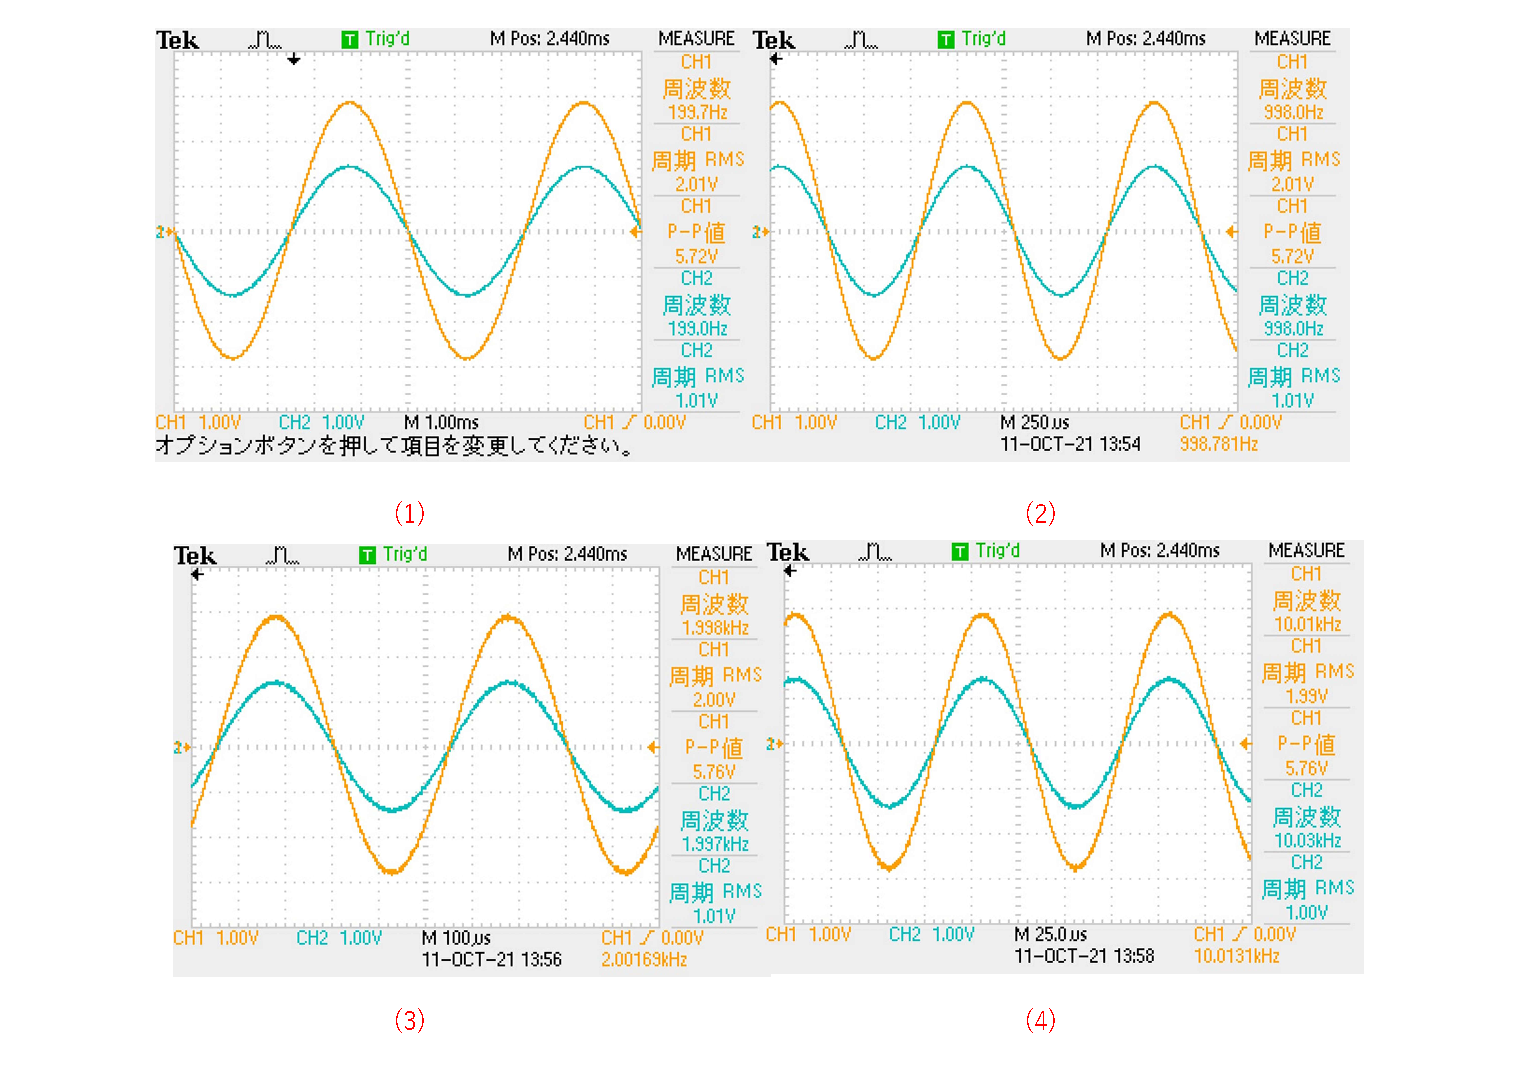
\includegraphics[keepaspectratio,scale=0.5]{Chapter11_osc_result.pdf}
	\caption{それぞれの周波数でのオシロスコープの出力画面}
\end{figure}
\rightline{次に続く→}

\newpage
表4.1にオシロスコープの出力結果を示す。表4.1のCH1では、発振器で設定した周波数 $f$と図3.1の回路図で流れてる周期RMS $V_{rms}$と、P-P値 $V_{pp}$の測定結果を示す。また表4.1のCH2では、発振器で設定した周波数$f$と図3.1の回路図で流れている周波数RMS $V_{rms}$の測定結果を示す。
\\\\
 なお、周波数$f$は$\SI{1}{\sec}$間に何周期することができるかというもので、以下の式から求めることができる[1]。(ここでは、周期を$T$とする。)
\begin{equation}
	f=\dfrac{1}{T}
\end{equation}
から求めることができる。周期RMS $V_{rms}$は電圧の最大値を$V_{max}$としたとき、
\begin{equation}
	V_{rms}=\dfrac{V_{max}}{\sqrt{2}}
\end{equation}
から求めることができる。またP-P値 $V_{pp}$とは、正弦波周期の電圧が正の最大値と負の最大値を足したものである。

\begin{table}[hbtp]
  \caption{オシロスコープの測定結果}
  \label{table:data_type}
  \centering
		\begin{tabular}{|cccccc|}
			\hline
			入力CHコネクタ    &                       &                        & 			測定値					 &                       &                                              \\ 
			\hline
			\hline
					CH1           & 周波数$f_1$/\si{\hertz} & $199.7$  & $998.0$  & $1.998$k & $10.01$k  \\ 
			  	              &    周期RMS $V_{rms1}$/V    & $2.01$   & $2.01$   & $2.00$  & $1.99$   \\
			                  &     P-P値 $V_{pp}$/V     & $5.72$   & $5.72$   & $5.76$  &	$5.76$ 	 \\
			\hline
			    CH2           & 周波数$f_2$/\si{\hertz} & $199.0$  & $998.0$  &	$1.997$k	& $10.03$k  \\
			                  &     周期RMS $V_{rms2}$/V    & $1.01$   & $1.01$		& $1.01$	&	$1.00$	 \\
			\hline  
		\end{tabular}
\end{table}
図4.1と表4.1から読み取れることは以下のとおりである。
\begin{itemize}
	\item 周波数を大きく変えたが、周期RMS $V_{rms}$との値は誤差レベルでしか、ずれていないことが分かる。
	\item 図4.1の(1)から(4)のどの波形でも、CH1とCH2の電圧の最大値の差が変わらない。
	\item  図4.1の(1)から(4)において、CH1の周期RMS $V_{rms}$の値は、どれもCH2の約2倍である。
\end{itemize}

%5.考察
\newpage
\section{考察}
今回の実験での考察は2つある。それを以下に(1)と(2)に示す。
\begin{itemize}
	\item [(1)]CH1の$V_{pp}$と発振器 $V$の関係\\最初に、P-P値 $V_{pp}$は4.実験結果にあるように、正弦波周期の電圧が正の最大値 $V_{max}$と負の最大値 $V_{min}$を足したものであることから、以下の式が成り立つ。
						\begin{equation}
							V_{pp}=V_{max}-V_{min}
						\end{equation}
						次に、各抵抗にかかる電圧の実効値を分圧の法則より求める。
						\begin{equation}
							V_{rms1}=\dfrac{VR_1}{R_1+R_2}
						\end{equation}
						\begin{equation}
							V_{rms2}=\dfrac{VR_2}{R_1+R_2}
						\end{equation}
						$V_{rms}$はキルヒホッフの第2法則より、以下のように求められる。
						\begin{equation}
							V_{rms}=V_{rms1}+V_{rms2}
						\end{equation}
						式(5.4)に式(5.2),(5.3)を代入すると以下の式が成り立つ。
						\begin{equation}
							\begin{split}
								&V_{rms}=\dfrac{VR_1}{R_1+R_2}+\dfrac{VR_2}{R_1+R_2}\\
								&\quad\quad=\dfrac{{VR_1}+{VR_2}}{{R_1+R_2}}\\
								&\quad\quad=\dfrac{V(R_1+R_2)}{{R_1+R_2}}\\
								&\quad\quad=V
							\end{split}
						\end{equation}
						よって、発振器$V$は実効値であると言える。
						次に、$V_{rms}$は式(4.2)より求められる。
						\begin{equation}
							V_{rms}=\dfrac{V_{max}}{\sqrt{2}}
						\end{equation}
						式(5.1)を式(5.6)に代入するために、式変形を行うと、
						\begin{equation}
							V_{max}=V_{pp}+V_{min}
						\end{equation}
						\begin{equation}
							V_{rms}=\dfrac{V_{pp}+V_{min}}{\sqrt{2}}
						\end{equation}
						を求められる。最後に、式(5.8)に式(5.5)の関係を適用すると、
						\begin{equation}
							V=\dfrac{V_{pp}+V_{min}}{\sqrt{2}}
						\end{equation}
						式(5.9)より、CH1 のVpp と発振器 Vの関係がわかる。また、式(5.9)に表4.1の測定値を代入すると、
						\begin{equation}
							V=\dfrac{5.72+(- \dfrac{5.72}{2})}{\sqrt{2}}=2.022
						\end{equation}
						\begin{equation}
							V=\dfrac{5.72+(- \dfrac{5.72}{2})}{\sqrt{2}}=2.022
						\end{equation}
						\begin{equation}
							V=\dfrac{5.76+(- \dfrac{5.76}{2})}{\sqrt{2}}=2.036
						\end{equation}
						\begin{equation}
							V=\dfrac{5.76+(- \dfrac{5.76}{2})}{\sqrt{2}}=2.036
						\end{equation}
						この時、式(5.10)~(5.13)はそれぞれ、周波数$f$の$\SI{199.7}{\hertz}$、$\SI{998.0}{\hertz}$、$\SI{1.998}{\kilo\hertz}$、$\SI{10.01}{\kilo\hertz}$の時の測定値で計算したものである。式(5.10)~(5.13)の計算結果より、発振器$V$はほぼ$\SI{2}{V}$あるため、測定値と設定値$\SI{2}{V}$であまり変わらないことが分かるため。よって、式(5.9)は成り立つと考えられる。


	\newpage			
	\item [(2)]CH1 $V_{rms1}$とCH2 $V_{rms2}$の周期RMS $V_{rms}$の関係\\図4.1のそれぞれの波形を見ると周波数が異なっているにもかかわらず、CH1では電圧の正の最大値と負の最大値が約2.9Vで、CH2では電圧の正の最大値と負の最大値が約1.4Vである。\\まずCH1とCH2の交流電圧を求める。ここで$V_{max1}$はCH1の電圧の最大値、$V_{max2}$はCH2の電圧の最大値である。
						\begin{equation}
							V_1=V_{max1}\sin(\omega t)
						\end{equation}
						\begin{equation}
							V_2=V_{max2}\sin(\omega t)
						\end{equation}
						式(5.14)と(5.15)にある、周波数$\omega$は同じ記号のため、周波数はそれぞれの交流電圧や電圧の最大値に影響しないことが分かる。また、周期RMSは以下のように求めることができる。
						\begin{equation}
							V_{rms}=\dfrac{V_{max}}{\sqrt{2}}
						\end{equation}
						式(5.16)を式(5.14)と(5.15)に代入するために、式変形をすると、
						\begin{equation}
								V_{max}=\sqrt{2} \times V_{rms}
						\end{equation}
						になり、式(5.17)を式(5.14)と(5.15)に代入すると、
						\begin{equation}
							V_1=\sqrt{2} \times V_{rms}\sin(\omega t)
						\end{equation}
						\begin{equation}
							V_2=\sqrt{2} \times V_{rms}\sin(\omega t)
						\end{equation}
						になる。式(5.16)より、周期RMS $V_{rms}$は電圧の正の最大値 $V_{max}$に比例して増えることが分かる。この事と、CH1はCH2に比べて最大値が2倍ということから、周期RMSも2倍であると言える。次に電圧はオームの法則より
						\begin{equation}
							V=RI
						\end{equation}
						から求めることができる。式(5.20)より、電圧は抵抗に比例することが分かるため、抵抗が2倍になると電圧も2倍になるということが分かる。またこの時、抵抗$R_1$$R_2$は共に$\SI{1}{\kilo\ohm}$である。そして、CH1の抵抗$R_1$$R_2$が接続されていて、CH2の抵抗は$R_2$のみが接続されている。このことから、CH1の抵抗値はCH2に比べて2倍である。\\
						よって
						電圧$V_1$は$V_2$より2倍であるといえる。電圧が2倍であると、式(5.18)、(5.19)よりCH1はCH2に比べて周期RMSが2倍になる。
\end{itemize}

%6.まとめ
\newpage
\section{まとめ}
今回の授業を通して、実験の目的である「オシロスコープを自在に扱えるように測定技術を習得する必要がある。」を達成することができたと思います。オシロスコープの機能を使って、波形を手動で位置調整し、CH1とCH2の位相を比較できるようになりました。しかし、図4.1では自分のオシロスコープの設定を間違えたことにより、X軸の1マスあたりの秒数をそろえることができていませんでした。このことから、図を大雑把に見たときに単純比較ができなくなってしまいました。次回からはこのようなことをなくすために、USBメモリに保存する前に、オシロスコープの確認作業を怠らないようにしたいと思います。

%7.参考文献
\section{参考文献}
1.山下 明、文系でもわかる電気回路、(株)翔泳社、2020年、P120・P130

\end{document}